%%%%%%%%%%%%%%%%%%%%%%%%%%%%%%%%%%%%%%%%%
% Masters/Doctoral Thesis 
% LaTeX Template
% Version 2.5 (27/8/17)
%
% This template was downloaded from:
% http://www.LaTeXTemplates.com
%
% Version 2.x major modifications by:
% Vel (vel@latextemplates.com)
%
% This template is based on a template by:
% Steve Gunn (http://users.ecs.soton.ac.uk/srg/softwaretools/document/templates/)
% Sunil Patel (http://www.sunilpatel.co.uk/thesis-template/)
%
% Template license:
% CC BY-NC-SA 3.0 (http://creativecommons.org/licenses/by-nc-sa/3.0/)
%
%%%%%%%%%%%%%%%%%%%%%%%%%%%%%%%%%%%%%%%%%

%----------------------------------------------------------------------------------------
%	PACKAGES AND OTHER DOCUMENT CONFIGURATIONS
%----------------------------------------------------------------------------------------

\documentclass[
12pt, % The default document font size, options: 10pt, 11pt, 12pt
oneside, % Two side (alternating margins) for binding by default, uncomment to switch to one side
english, % ngerman for German
onehalfspacing, % Single line spacing, alternatives: onehalfspacing or doublespacing
%draft, % Uncomment to enable draft mode (no pictures, no links, overfull hboxes indicated)
%nolistspacing, % If the document is onehalfspacing or doublespacing, uncomment this to set spacing in lists to single
liststotoc, % Uncomment to add the list of figures/tables/etc to the table of contents
%toctotoc, % Uncomment to add the main table of contents to the table of contents
%parskip, % Uncomment to add space between paragraphs
%nohyperref, % Uncomment to not load the hyperref package
headsepline, % Uncomment to get a line under the header
%chapterinoneline, % Uncomment to place the chapter title next to the number on one line
consistentlayout, % Uncomment to change the layout of the declaration, abstract and acknowledgements pages to match the default layout
]{MastersDoctoralThesis} % The class file specifying the document structure
\setcounter{tocdepth}{3} % Uncomment this and next line to enable numbering of subsubsections 
\setcounter{secnumdepth}{3}
\usepackage[utf8]{inputenc} % Required for inputting international characters
\usepackage[T1]{fontenc} % Output font encoding for international characters
\usepackage{todonotes}
\usepackage{mathpazo} % Use the Palatino font by default

%\usepackage[style=numeric]{biblatex} % Use the bibtex backend with the authoryear citation style (which resembles APA)
\usepackage[backend=bibtex,style=numeric]{biblatex}
%\usepackage[backend=bibtex,style=authoryear]{biblatex} % this will use author and year for in text referencing
\bibliography{main}
\bibliography{honoursThesis} 
\usepackage[autostyle=true]{csquotes} % Required to generate language-dependent quotes in the bibliography
\usepackage{amsmath} % Allows for the use of multi-line and aligned equations

%----------------------------------------------------------------------------------------
%	MARGIN SETTINGS
%----------------------------------------------------------------------------------------

\geometry{
	paper=a4paper, % Change to letterpaper for US letter
	inner=2.5cm, % Inner margin
	outer=3.8cm, % Outer margin
	bindingoffset=.5cm, % Binding offset
	top=1.5cm, % Top margin
	bottom=1.5cm, % Bottom margin
	%showframe, % Uncomment to show how the type block is set on the page
}

%----------------------------------------------------------------------------------------
%	THESIS INFORMATION
%----------------------------------------------------------------------------------------

\thesistitle{Local GPS Spoofing using a Software Defined Radio} % Your thesis title, this is used in the title and abstract, print it elsewhere with \ttitle
\supervisor{Dr. Saeed \textsc{Rehman}} % Your supervisor's name, this is used in the title page, print it elsewhere with \supname
\examiner{} % Your examiner's name, this is not currently used anywhere in the template, print it elsewhere with \examname
\degree{Bachelour of Engineering(Electrical and Electronic)(Honours)} % Your degree name, this is used in the title page and abstract, print it elsewhere with \degreename
\author{Alastair \textsc{Wiegelmann}} % Your name, this is used in the title page and abstract, print it elsewhere with \authorname
\addresses{} % Your address, this is not currently used anywhere in the template, print it elsewhere with \addressname

\subject{Electronic/Communication Engineering} % Your subject area, this is not currently used anywhere in the template, print it elsewhere with \subjectname
\keywords{Communication, GPS, Spoofing, Modulation} % Keywords for your thesis, this is not currently used anywhere in the template, print it elsewhere with \keywordnames
\university{\href{https://www.flinders.edu.au/}{Flinders University}} % Your university's name and URL, this is used in the title page and abstract, print it elsewhere with \univname
\department{\href{https://www.flinders.edu.au/college-science-engineering}{College of Science and Engineering}} % Your department's name and URL, this is used in the title page and abstract, print it elsewhere with \deptname
\group{} % Your research group's name and URL, this is used in the title page, print it elsewhere with \groupname
\faculty{\href{}{}} % Your faculty's name and URL, this is used in the title page and abstract, print it elsewhere with \facname

\AtBeginDocument{
\hypersetup{pdftitle=\ttitle} % Set the PDF's title to your title
\hypersetup{pdfauthor=\authorname} % Set the PDF's author to your name
\hypersetup{pdfkeywords=\keywordnames} % Set the PDF's keywords to your keywords
}

\begin{document}

\frontmatter % Use roman page numbering style (i, ii, iii, iv...) for the pre-content pages

\pagestyle{plain} % Default to the plain heading style until the thesis style is called for the body content

%----------------------------------------------------------------------------------------
%	TITLE PAGE
%----------------------------------------------------------------------------------------

\begin{titlepage}
\begin{center}

\vspace*{.06\textheight}
{\scshape\LARGE \univname\par}\vspace{1.5cm} % University name
\textsc{\Large Honours Thesis}\\[0.5cm] % Thesis type

\HRule \\[0.4cm] % Horizontal line
{\huge \bfseries \ttitle\par}\vspace{0.4cm} % Thesis title
\HRule \\[1.5cm] % Horizontal line
 
\begin{minipage}[t]{0.4\textwidth}
\begin{flushleft} \large
\emph{Author:}\\
{\authorname} % Author name - remove the \href bracket to remove the link
\end{flushleft}
\end{minipage}
\begin{minipage}[t]{0.4\textwidth}
\begin{flushright} \large
\emph{Supervisor:} \\
{\supname} % Supervisor name - remove the \href bracket to remove the link  
\end{flushright}
\end{minipage}\\[3cm]
 
\vfill

\large \textit{A thesis submitted in fulfilment of the requirements\\ for the degree of \degreename}\\[0.3cm] % University requirement text
%%\groupname\\\deptname\\[2cm] % Research group name and department name
 
\vfill

{\large \today}\\[4cm] % Date
%\includegraphics{Logo} % University/department logo - uncomment to place it
 
\vfill
\end{center}
\end{titlepage}

%----------------------------------------------------------------------------------------
%	DECLARATION PAGE
%----------------------------------------------------------------------------------------

\begin{declaration}
\addchaptertocentry{\authorshipname} % Add the declaration to the table of contents
\noindent I, \authorname, declare that this thesis titled, \enquote{\ttitle} and the work presented in it are my own. I confirm that:

\begin{itemize} 
\item This work was done wholly while in candidature for a degree of \degreename.
\item This document is in accordance with the plagiarism policy of \univname.
\item Where any part of this thesis has previously been submitted for a degree or any other qualification at this University or any other institution, this has been clearly stated.
\item Where I have consulted the published work of others, this is always clearly attributed.
\item Where I have quoted from the work of others, the source is always given. With the exception of such quotations, this thesis is entirely my own work.
\item I have acknowledged all main sources of help.
\item Where the thesis is based on work done by myself jointly with others, I have made clear exactly what was done by others and what I have contributed myself.\\
\end{itemize}
 
\noindent Signed:\\
\rule[0.5em]{25em}{0.5pt} % This prints a line for the signature
 
\noindent Date:\\
\rule[0.5em]{25em}{0.5pt} % This prints a line to write the date
\end{declaration}

\cleardoublepage

%----------------------------------------------------------------------------------------
%	QUOTATION PAGE
%----------------------------------------------------------------------------------------

% \vspace*{0.2\textheight}

% \noindent\enquote{\itshape One of the major problems encountered in time travel is not that of becoming your own father or mother. There is no problem in becoming your own father or mother that a broad-minded and well-adjusted family can't cope with. There is no problem with changing the course of history—the course of history does not change because it all fits together like a jigsaw. All the important changes have happened before the things they were supposed to change and it all sorts itself out in the end.

% The major problem is simply one of grammar, and the main work to consult in this matter is Dr. Dan Streetmentioner's Time Traveler's Handbook of 1001 Tense Formations. It will tell you, for instance, how to describe something that was about to happen to you in the past before you avoided it by time-jumping forward two days in order to avoid it. The event will be descibed differently according to whether you are talking about it from the standpoint of your own natural time, from a time in the further future, or a time in the further past and is futher complicated by the possibility of conducting conversations while you are actually traveling from one time to another with the intention of becoming your own mother or father.

% Most readers get as far as the Future Semiconditionally Modified Subinverted Plagal Past Subjunctive Intentional before giving up; and in fact in later aditions of the book all pages beyond this point have been left blank to save on printing costs.

% The Hitchhiker's Guide to the Galaxy skips lightly over this tangle of academic abstraction, pausing only to note that the term "Future Perfect" has been abandoned since it was discovered not to be.}\bigbreak

% \hfill The Hitch Hiker's Guide To The Galaxy

%----------------------------------------------------------------------------------------
%	ABSTRACT PAGE
%----------------------------------------------------------------------------------------

\begin{abstract}
  \addchaptertocentry{\abstractname} % Add the abstract to the table of contents

\end{abstract}

%----------------------------------------------------------------------------------------
%	ACKNOWLEDGEMENTS
%----------------------------------------------------------------------------------------

\begin{acknowledgements}
\addchaptertocentry{\acknowledgementname} % Add the acknowledgements to the table of contents
I wish to thank all those that have supported me through not only my thesis, but my entire degree.
\end{acknowledgements}

%----------------------------------------------------------------------------------------
%	LIST OF CONTENTS/FIGURES/TABLES PAGES
%----------------------------------------------------------------------------------------

\tableofcontents % Prints the main table of contents

\listoffigures % Prints the list of figures

\listoftables % Prints the list of tables

%----------------------------------------------------------------------------------------
%	ABBREVIATIONS
%----------------------------------------------------------------------------------------

\begin{abbreviations}{ll} % Include a list of abbreviations (a table of two columns)

\textbf{BOC} & \textbf{B}inary \textbf{O}ffset \textbf{C}arrier\\
\textbf{BPSK} & \textbf{B}inary \textbf{P}hase-\textbf{S}hift \textbf{K}eying\\
\textbf{CDMA} & \textbf{C}ode \textbf{D}ivision \textbf{M}ultiple \textbf{A}ccess\\
\textbf{COTS} & \textbf{C}ommerical \textbf{O}ff \textbf{T}he \textbf{S}helf\\
\textbf{DSP} & \textbf{D}igital \textbf{S}ignal \textbf{P}rocessing\\
\textbf{EGA} & \textbf{E}uropean \textbf{G}NSS \textbf{A}gency\\
\textbf{EM} & \textbf{E}lectro\textbf{M}agnetic\\
\textbf{ESA} & \textbf{E}uropean \textbf{S}pace \textbf{A}gency\\
\textbf{FDMA} & \textbf{F}requency \textbf{D}ivision \textbf{M}ultiple \textbf{A}ccess\\
\textbf{GLONASS} & \textbf{GLO}bal \textbf{NA}vigation \textbf{S}atellite \textbf{S}ystem\\
\textbf{GNSS} & \textbf{G}lobal \textbf{N}avigation \textbf{S}atellite \textbf{S}ystem\\
\textbf{GPS} & \textbf{G}lobal \textbf{P}ositioning \textbf{S}ystem\\
\textbf{IRNSS} & \textbf{I}ndian \textbf{R}eginal \textbf{N}avigation \textbf{S}atellite \textbf{S}ystem\\
\textbf{LEO} & \textbf{L}ow \textbf{E}arth \textbf{O}rbit\\
\textbf{MEO} & \textbf{M}edium \textbf{E}arth \textbf{O}rbit\\
\textbf{NavIC} & \textbf{Nav}igation (with) \textbf{I}ndian \textbf{C}onstellation\\
\textbf{NMEA} & \textbf{N}ational \textbf{M}arine \textbf{E}lectronics \textbf{A}ssociation \\
\textbf{OSNMA} & \textbf{O}pen \textbf{S}ervice \textbf{N}avigation \textbf{M}essage \textbf{A}uthentication\\
\textbf{PNT} & \textbf{P}osition, \textbf{N}avigation and \textbf{T}iming\\
\textbf{PVT} & \textbf{P}osition, \textbf{V}elocity and \textbf{T}iming\\
\textbf{QFSS} & \textbf{Q}uasi-\textbf{Z}enith \textbf{S}atellite \textbf{S}ystem\\
\textbf{RF} & \textbf{R}adio \textbf{F}requency\\
\textbf{RHCP} & \textbf{R}ight \textbf{H}and \textbf{C}ircular \textbf{P}olarisation\\
\textbf{SDR} & \textbf{S}oftware \textbf{D}efined \textbf{R}adio\\
\textbf{SNR} & \textbf{S}ignal (to) \textbf{N}oise \textbf{R}atio\\
\textbf{SPS} & \textbf{S}amples \textbf{P}er \textbf{S}econd\\
\textbf{UAV} & \textbf{U}nmanned \textbf{A}erial \textbf{V}ehicle\\
\textbf{V2V} & \textbf{V}ehicle (to) \textbf{V}ehivle (communication)\\
\textbf{V2X} & \textbf{V}ehicle (to) (everything) (communication)\\
\textbf{XML} & e\textbf{X}tensible \textbf{M}arkup \textbf{L}anguage\\
\textbf{WSF} & \textbf{W}hat (it) \textbf{S}tands \textbf{F}or\\

\end{abbreviations}

%----------------------------------------------------------------------------------------
%	PHYSICAL CONSTANTS/OTHER DEFINITIONS
%----------------------------------------------------------------------------------------

\begin{constants}{lr@{${}={}$}l} % The list of physical constants is a three column table

% The \SI{}{} command is provided by the siunitx package, see its documentation for instructions on how to use it

Speed of Light & $c_{0}$ & \SI{2.99792458e8}{\meter\per\second} (exact)\\
Standard Gravitational Parameter of Earth & $\mu_{earth}$ & \SI{3.986004418e14}{\meter\cubed\per\second\squared} \\
Constant Name & $Symbol$ & $Constant Value$ with units\\

\end{constants}

%----------------------------------------------------------------------------------------
%	SYMBOLS
%----------------------------------------------------------------------------------------

\begin{symbols}{lll} % Include a list of Symbols (a three column table)

$a$ & distance & \si{\meter} \\
$P$ & power & \si{\watt} (\si{\joule\per\second}) \\
Symbol & Name & Unit \\

\addlinespace % Gap to separate the Roman symbols from the Greek

$\omega$ & angular frequency & \si{\radian} \\
$\mu$ & standard gravitational parameter & \si{m^3s^{-2}}

\end{symbols}

%----------------------------------------------------------------------------------------
%	DEDICATION
%----------------------------------------------------------------------------------------

%\dedicatory{For/Dedicated to/To my\ldots} 

%----------------------------------------------------------------------------------------
%	THESIS CONTENT - CHAPTERS
%----------------------------------------------------------------------------------------

\mainmatter % Begin numeric (1,2,3...) page numbering

\pagestyle{thesis} % Return the page headers back to the "thesis" style

% Include the chapters of the thesis as separate files from the Chapters folder
% Uncomment the lines as you write the chapters

% Chapter Template

\chapter{Introduction}\label{chapter:firstchapter} % Main chapter title

\label{Chapter1} % Change X to a consecutive number; for referencing this chapter elsewhere, use \ref{ChapterX}

%----------------------------------------------------------------------------------------
%	SECTION 1
%----------------------------------------------------------------------------------------
\section{Motivation}\label{sec:Motivation}

% It is a good idea to have each sentence on a separate line, so that if you get feedback or changes from someone else
% the diffs will be much easier to manage

As society moves through the age of technology there is an exponential reliance on reliable access to position and time data. The main source of this infomation over the
recent decades has been through GNSS constellations. GNSS services are now tightly integrated with many facets of life from personal navigation, public transport and
management of energy infrastructure. This has made these services the target of attacks. In order to provide adequete defence knowledge of how the attacks are performed is
required.

As it currently stands there is no active research or efforts to do so from within \univname. Therefore, to ensure that Flinders is able to keep up with moving trends and
ever advancing technology this project was devised. This thesis will document background information on both GNSS operating principles as well as background research in
spoofing. A workflow was generated and will be used as a starting point for continual research.

\section{Aims and Benefits}\label{sec:Aims}
The aims of this thesis are to investigate and perform a GPS spoofing attack in order to gain a better understanding of the operation of the GPS infrastructure and attack
methodology. This will be used to create a baseline for SDR capabilities reasearch from within \univname where future reasearch can build upon this inital documentation.
The depth of research into the most cutting edge SDR and GPS Spoofing technologies will therefore not be covered in this paper but will be the topic of future research
within the College of Science and Engineering at \univname.
There will be some emphasis placed on the technical knowledge requried to perform such attacks and the cost of performing them now as opposed to the past. This will
allow for further work in counter-measures of GPS spoofing.
This thesis will purely concentrate on the research of and implementation of a spoofing device. There will be no implementation of anti-spoofing methodology.

\emph{relate this to the electronic warefare department / chair here at flinders. GPS SPoofing/jamming is one part of this section that can be used by students for research or testing.}

\section{Research Questions}\label{sec:RQs}
\begin{enumerate}
    \item What resources are required to perform a spoofing attack on commercial GPS receiver?
    \item What effort and technical expertise is required for a spoofing attack on a commercial GPS receiver?
    \item How can a prototype GPS spoofer be implemented in a controlled environment?
    \item How could a prototype be implemented in a real-time static or dynamic environment? 
\end{enumerate}

\section{Limitations}\label{sec:Limits}
Due to hardware and software limitations, all testing will be performed on the Navstar GPS system only. There will be no multi constellation. However the theory and basic
structure of the attacks are relevant to all constellations since the same trilateration technique is common to them all.

Since GPS and more speficically the L1 frequency band of GPS is so ubiquitous in society there is open source software available that made this project achieveable. While
it would be possilbe to extend the project to encompass other constellations and frequency bands, this would require much more time that is allowed for.

\section{Thesis Structure}\label{sec:structure}
The rest of this thesis will have a structure as follows, Chapter \ref{Chapter2} will introduce the history and concepts in GNSS technology as well as defining and
introducing GNSS spoofing. Chapter \ref{Chapter3} provides a summary of relevant research in the area of GNSS spoofing attacks and defences. Spoof defence will include
detection and mitigation. Chapter \ref{Chapter4} outlines the method used in the spoofing attack. Chapter \ref{Chapter5} will show the results gathered from the
experimentation. Chapter \ref{Chapter6} will provide discussion regarding the results of the experiments as well as issues and solutions encoutered while performing the
experiments as well as recommendations for future work. Finally chapter \ref{Chapter7} willl provide a conclusion to the project.
% Chapter Template

\chapter{Introduction to GNSS Systems} % Main chapter title

\label{Chapter2} % Change X to a consecutive number; for referencing this chapter elsewhere, use \ref{ChapterX}

%----------------------------------------------------------------------------------------
%	SECTION 1
%----------------------------------------------------------------------------------------

\section{History of GNSS Systems}
\emph{In 2021 there are many different GNSS systems that are in place that service the globe. It is a technology that has become deeply ingrained in the everyday lives of
most people around the world. The first form of navigation system that was used by populatinons around the world was using the stats as a type of map. The first digital
based navigation system similar to what we know today was the use of terrestrial based radio transmitters. The concept was similar to that of the current satellite based
systems although the accuracy was far lower than is acceptable today. The USA developed and commissioned the first satellite based nanvigation system}

As of 2021 there are six operational GNSS systems in use. These are GPS (USA), GLONASS (Russia), Galileo (EU), BeiDou (China), IRNSS (India) and QZSS (Japan). The QZSS
system currently acts to complement the coverage of GPS in the East Asian and Oceanic regions with 4 operational satellites. There are plans to increase this number of
satellites to allow for stand alone use as a GNSS provider. 
GNSS, more specifically GPS, dates back to 1957 during the space race with then USSR \cite{RN43}. 

When Russian satellite Sputnik 1 was launched scientists at the John Hopkins University were able to
track its position and velocity by measuring the doppler shift of the craft. This tracking from Doppler shift measurements contniued with the launch of the subsequent
satellites Sputnik 2 and Explorer 1. After this it was thought that the process could be reversed such that a satellite with a known position could be used to resolve an
unknown position on earth. In the 1960's the TRANSIT satellite navigation system was made operational for US Navy use, mainly for postion and navigation of nuclear
ballistic missile submarines. TRANSIT received strong support due to the accuracy of up to 80ft (24m) which was a significant improvement over existing VLF (Very Low
Frequency) hyperbolic navigation systems. After 32 years of operation the system was retired in 1996 after proving that space crafts could be reliable \cite{RN45}. 

In 1973 the US combined two existing programmes in TIMATION and 'Project 621B' to form the 'NAVSTAR Global Positioning System' which would later become known more
commonly as GPS. The initial intention for the use of GPS was for military only. However, in 1983 there was an incident that saw a Korean Airlines flight shot down by a
Soviet fighter mistaking it for a US aircraft when it wandered off course. After this incident President Reagen announced that GPS would be made available for civilian
use. The military insisted that the accuracy of the system be purposley degraded for civilian use though selective availabililty such that GPS could not be used by
adversaries. In 1993 the system was declared operational. To combat the intentional accuracy reduction of the GPS system augmentation systems started to appear. Soon
after there were Government funded versions of DGPS (Differetial GPS) systems \cite{RN43}. The significantly increases the accuracy by using a receiver with a knwon location and
having that reciever calculate its position from the satellite signals and compare with the known position. The corrections are then broadcast. 

The soviet union launched their first GLONASS satellite in 1982, and in the following three years 10 more were launched. There were some technical differences between the
GLONASS and GPS constellations. The orbital planes were different and GLONASS uses an FDMA (Frequency Division Multiple Access) scheme as opposed to the GPS CDMA (Code
Division Multiple Access). In 1993 president Yeltsin declared that the GLONASS constllation was fully operational, however this was not the case. 


\todo{add graph: x axis year y axis accuracy}  
% Chapter Template

\chapter{Methodology} % Main chapter title

\label{Chapter3} % Change X to a consecutive number; for referencing this chapter elsewhere, use \ref{ChapterX}
%\medskip
Summary of testing:
\begin{itemize}
    \item Used commercial GPS receiver to check received SNR values \\ Antennae used:
    \begin{itemize}
        \item passive patch antenna
        \item active antenna
        \item Log-periodic antenna
    \end{itemize}
    This resulted in a preliminary finding that the active antenna improved signal to noise ratio by 8dB. \todo{Update with more formal findings}
    \item Use SDR + GNSS-SDR to receive similar signals and compare SNR values
    \item Use stored text file of gps data and connect Tx to Rx antenna port (via attenuator) to check if programs are manipulating the data as they should be.
    \item Use stored txt file of gps data (received from commercial receiver) and transmit gps signal using log periodic antenna to see if phone GPS can be spoofed into thinking it is in another geographical location.
\end{itemize}
\medskip
All of the software packages used are free and opensource.
List of Software packages used:
\begin{itemize}
    \item GNURadio
    \item GNSS-SDR
    \item GNSS-SDR-monitor
    \item gps-sdr-sim
\end{itemize}

\textbf{It would be great to be able to perform a meaconing attack. This requries real time reception and rebroadcast with a higher power. The extra time delay
makes the spoofing victim believe they are elsewhere. This should be a search term.}

%----------------------------------------------------------------------------------------
%	SECTION 1
%----------------------------------------------------------------------------------------

\section{Testing Methodology}

In this section the method of creating a GPS signal spoofing device is detailed. The main part of this project is the upgradability of the SDR platform
and in particular the USRP N210 SDR. As previously mentioned the benefit of using an SDR over using an ASIC is that with a new version of software 
new capacilities are availeble to the device. This could be benefitial to either the spoofer or spoof defense. 

%-----------------------------------
%	SUBSECTION 1
%-----------------------------------
\subsection{Subsection 1}

Nunc posuere quam at lectus tristique eu ultrices augue venenatis. Vestibulum ante ipsum primis in faucibus orci luctus et ultrices posuere cubilia Curae; Aliquam erat volutpat. Vivamus sodales tortor eget quam adipiscing in vulputate ante ullamcorper. Sed eros ante, lacinia et sollicitudin et, aliquam sit amet augue. In hac habitasse platea dictumst.

%-----------------------------------
%	SUBSECTION 2
%-----------------------------------

\subsection{Subsection 2}
Morbi rutrum odio eget arcu adipiscing sodales. Aenean et purus a est pulvinar pellentesque. Cras in elit neque, quis varius elit. Phasellus fringilla, nibh eu tempus venenatis, dolor elit posuere quam, quis adipiscing urna leo nec orci. Sed nec nulla auctor odio aliquet consequat. Ut nec nulla in ante ullamcorper aliquam at sed dolor. Phasellus fermentum magna in augue gravida cursus. Cras sed pretium lorem. Pellentesque eget ornare odio. Proin accumsan, massa viverra cursus pharetra, ipsum nisi lobortis velit, a malesuada dolor lorem eu neque.

%----------------------------------------------------------------------------------------
%	SECTION 2
%----------------------------------------------------------------------------------------

\section{Main Section 2}

Sed ullamcorper quam eu nisl interdum at interdum enim egestas. Aliquam placerat justo sed lectus lobortis ut porta nisl porttitor. Vestibulum mi dolor, lacinia molestie gravida at, tempus vitae ligula. Donec eget quam sapien, in viverra eros. Donec pellentesque justo a massa fringilla non vestibulum metus vestibulum. Vestibulum in orci quis felis tempor lacinia. Vivamus ornare ultrices facilisis. Ut hendrerit volutpat vulputate. Morbi condimentum venenatis augue, id porta ipsum vulputate in. Curabitur luctus tempus justo. Vestibulum risus lectus, adipiscing nec condimentum quis, condimentum nec nisl. Aliquam dictum sagittis velit sed iaculis. Morbi tristique augue sit amet nulla pulvinar id facilisis ligula mollis. Nam elit libero, tincidunt ut aliquam at, molestie in quam. Aenean rhoncus vehicula hendrerit.
% Chapter Template
\chapter{Methodology} % Main chapter title

\label{Chapter4} % Change X to a consecutive number; for referencing this chapter elsewhere, use \ref{ChapterX}

This chapter covers the hardware and software setup used for performing the GPS spoofing experimnentations. Rationalising the choises made and discussing the benefits and
limitations of these selections.

%----------------------------------------------------------------------------------------
%	SECTION 1
%----------------------------------------------------------------------------------------

\section{Testing Methodology}

In this section the method of creating a GPS signal spoofing device is detailed. The main part of this device is the upgradability of the SDR platform
and in particular the USRP N210 SDR. As previously mentioned the benefit of using an SDR over using an ASIC is that with a new version of software 
new capacilities are availeble to the device. This could be benefitial to either the spoofer or spoof defense. 

The success of the spoofing was dictated by whether the receiver was able to lock onto the signal and calculate the same location as expected or travel the same path
depending on whether the test is a satic or dynamic spoofing test. 

Testing was also performed on the reception of GPS signals. Such that they could be used in Meaconing attacks. Initally there was an attempt to receive a GPS signal using
the GPS-SDR software as proof that the antennae were operational. This was then changed such that the reception was handled directly through GNURadio and the raw
digitised version of the signal was saved to a file such that it could be replayed elsewhere.

%----------------------------------------------------------------------------------------
%	SECTION 2
%----------------------------------------------------------------------------------------

\section{Data Collection}

To see the effectiveness of the GPS spoofing methods experiments were carried out and results were recoreded. The success of the experiments were dictated by whether or
not the receiver was reporting false location or timing information. Using an adroid phone there is access to the raw GPS information which can be used to determine if
the spoofing signal is being accepted. However, the use of a "maps" program was also used as a way to determine if there was any form of software/hardware anti-spoofing
technique being used post gps receiver. A simple COTS was also used to log the NMEA sentences from its serial interface. A custom program was generated in order to graph
various outputs from these sentences.

For the purpose of this project just three sentences were used when parsing the log files, "GPGGA", "GPGSV" and "GPRMC". The GP mnemonic is a designation that the
received signal was from GPS. The other constellations have their own designations when using NMEA sentences as dictated by Table \ref{tab:NMEA Mnemonics}. 
GGA (Global Positioning System Fix Data) \footnote{https://www.nmea.org/Assets/20130801 0183 identifier list.pdf} sentences contain information related to the fix of the
GPS signal. The calcaulted latitude and longitude as well as whether DGPS is being used in the fix, as well as others, as shown in Table \ref{tab:NMEA GGA Struct}.  

An example of a GGA sentence is:
\begin{verbatim}
$GPGGA,000056.000,3500.5533,S,13834.1337,E,1,10,0.87,-14.7,M,-0.7,M,,*74
\end{verbatim}

\renewcommand{\arraystretch}{1.5}
\begin{table}
    \begin{center}
        \caption{NMEA GGA Sentence structure}
        \label{tab:NMEA GGA Struct}
        \begin{tabular}{ |m{4cm}|c|p{6cm}| }
            \hline
            \textbf{Field} & \textbf{Example} & \textbf{Description} \\
            \hline
            Message ID & \$GPGGA & GGA Protocol header \\
            \hline
            UTC time & 000056.000 & hhmmss.sss \\
            \hline
            Latitude & 3500.5533 & ddmm.mmmm \\
            \hline
            N/S Indicator & S & N = North, S = South\\
            \hline
            Longitude & 13834.1337 & dddmm.mmmm \\
            \hline
            E/W Indicator & E & E = East, W = West\\
            \hline
            Position Fix Indicator & 1 & 0: Fix not available \newline 1: GPS SPS mode, fix valid \newline 2: DGPS SPS mode, fix valid\\
            \hline
            Sattelites used & 10 & \\
            \hline
            HDOP & 0.87 & Horizontal dilution of precision\\
            \hline
            MLS Altitude & -14.7 & Meters \\
            \hline
            Units & M & Meters \\
            \hline
            Geoid separation & -0.7 & Meters \\
            \hline
            Units & M & Meters\\
            \hline
            Age of differential correlation & & Seconds\\
            \hline
            Differential reference station ID & &  \\
            \hline
            Checksum & *74 &  \\
            \hline
            <CR><LF> & & End of message termination \\
            \hline
        \end{tabular}
    \end{center}
\end{table}
\renewcommand{\arraystretch}{1}

The use of GSV (GNSS Satellites in View) sentences allowed for tracking how many and which satellites were in view (SVID) and what the $\frac{C}{N_0}$ ratio was. This was used to generate the carrier to
noise graphs. Since the sentences can only be a set length as per the standard, multiple successive GSV sentences may need to be sent.

An example of a GSV sentence that is part of a group of 4 is:
\begin{verbatim}
$GPGSV,4,1,13,23,70,156,52,10,69,284,52,20,50,138,,18,49,117,52*73
$GPGSV,4,2,13,27,37,224,52,16,32,276,52,15,26,127,51,26,23,308,51*77
$GPGSV,4,3,13,29,19,038,17,32,18,001,18,44,05,279,,13,02,148,47*75
$GPGSV,4,4,13,193,,,*40
\end{verbatim}

\renewcommand{\arraystretch}{1.5}
\begin{table}
    \begin{center}
        \caption{NMEA GSV Sentence structure}
        \label{tab:NMEA GSV Struct}
        \begin{tabular}{ |m{4cm}|c|p{6cm}| }
            \hline
            \textbf{Field} & \textbf{Example} & \textbf{Description} \\
            \hline
            Message ID & \$GPGSV & GSV Protocol header \\
            \hline
            Number of messages & 4 & Number of messages in group \\
            \hline
            Sequence Number & 1 & Message number \\
            \hline
            Satellites in view & 13 & Total number of satellites in view\\
            \hline
            Satellite ID 1 & 23 & PRN number of satellite \\
            \hline
            Elevation 1 & 70 & Elevation in degrees (0-90)\\
            \hline
            Azimuth 1 & 156 & Azimuth in degrees (0-359)\\
            \hline
            SNR 1 & 52 & SNR in dBHz (0-99)\\
            \hline
            Satellite ID 2 & 10 & PRN number of satellite \\
            \hline
            Elevation 2 & 69 & Elevation in degrees (0-90)\\
            \hline
            Azimuth 2 & 284 & Azimuth in degrees (0-359)\\
            \hline
            SNR 2 & 52 & SNR in dBHz (0-99)\\
            \hline
            Satellite ID 3 & 20 & PRN number of satellite \\
            \hline
            Elevation 3 & 50 & Elevation in degrees (0-90)\\
            \hline
            Azimuth 3 & 138 & Azimuth in degrees (0-359)\\
            \hline
            SNR 3 &  & SNR in dBHz (0-99)\\
            \hline
            Satellite ID 4 & 18 & PRN number of satellite \\
            \hline
            Elevation 4 & 49 & Elevation in degrees (0-90)\\
            \hline
            Azimuth 4 & 117 & Azimuth in degrees (0-359)\\
            \hline
            SNR 4 & 52 & SNR in dBHz (0-99)\\
            \hline
            Checksum & *73 &  \\
            \hline
            <CR><LF> & & End of message termination \\
            \hline
        \end{tabular}
    \end{center}
\end{table}
\renewcommand{\arraystretch}{1}

RMC (Recommended Minimum Specific GNSS Data)

\begin{verbatim}
$GPRMC,000118.000,A,3500.4918,S,13834.1369,E,53.66,12.07,300321,,,A*78
\end{verbatim}

\renewcommand{\arraystretch}{1.5}
\begin{table}
    \begin{center}
        \caption{NMEA RMC Sentence structure}
        \label{tab:NMEA RMC Struct}
        \begin{tabular}{ |m{4cm}|c|p{6cm}| }
            \hline
            \textbf{Field} & \textbf{Example} & \textbf{Description} \\
            \hline
            Message ID & \$GPRMC & RMC Protocol header \\
            \hline
            UTC time & 000118.000 & hhmmss.sss \\
            \hline
            Status & A & A = Valid, V = Not Valid \\
            \hline
            Latitude & 3500.4918 & ddmm.mmmm\\
            \hline
            N/S Indicator & S & N = North, S = South\\
            \hline
            Longitude & 13834.1369 & dddmm.mmmm \\
            \hline
            E/W Indicator & E & E = East, W = West\\
            \hline
            Speed over ground & 53.66 & knots \\
            \hline
            Course over ground & 12.07 & degrees \\
            \hline
            HDOP & 0.87 & Horizontal dilution of precision\\
            \hline
            Date & 300321 & ddmmyy \\
            \hline
            Magnetic Variation &  & Meters \\
            \hline
            Mode & A & A = Autonomous, D = DGPS, E = DR \\
            \hline
            Checksum & *78 &  \\
            \hline
            <CR><LF> & & End of message termination \\
            \hline
        \end{tabular}
    \end{center}
\end{table}
\renewcommand{\arraystretch}{1}

\section{Hardware Setup}
For all experiments the same hardware was used. This included the USRP SDR, laptop and GPS receiver. The laptop was an important piece of eqiupment since it needed to be
powerful enough to be able to feed the data to the SDR quick enough to avoid the aformentioned underrun issues. Towards the end of the project there was a hardware fault
with the Pixel XL phone receiver. This was replaced by the Pixel 4a 5G.

There was no formal decision process for choosing the hardware components since they were all parts that had already been purchased and were in possesion of the
supurvisor. Having said that some research went into the suitabilty of the equipment, mainly the SDR. It was found that this was one of the most powerful and most
importantly had one of the most stable clock osiclators availble in software defined radios. This made is well suited to GNSS based tasks. Alternatives, like the
RTL-SDR are capable devices for the cost, but only offer reception. Duplex options like the HackRF are also suitable for transmitting high bandwidth signals, however the
on board clock is not stable enough for highly accurate signals like that of GNSS. There was a workaround for this, which included desoldering the included oscillator and
soldering a more stable part. In future, if access to USRP based SDR's is not availble then this would be a very good second option. However, there was access to a better
tool, being the N210, therfore it was chosen. From Ettus, there were two daughtercards that allow access to the desired 1575.42MHz band of the L1 GPS signal, the SBX and
WBX. The SBX was chosen because it was already available. It should be noted that there would be no theoretical difference between either daughtercard since the desired
freqeuency was not at the extreme of either cards bands. Either card would also be capable of transmitting or receiving on the other bands of GNSS constellations.

To ensure the SDR and PC were able to communicate, an ehternet cable was connected between each device and the IP address of the PC was set to 192.168.0.2/24 as per the
default configuration from the setup documanetation. To check if the IP address was correctly set, a command line program was run that would pole the appropriate
interfaces of the PC and check for USRP devices attached. \todo{insert image of UHD FIND DEVICES}. There was also a command line program that allowed for the probing of a
radio to gatehr information on what daughtercard was installed and other propertiues. \todo{inset image}.

\begin{itemize}
    \item Laptop
    \begin{itemize}
        \item Dell Inspiron 15
        \item CPU: Core i7 Quad Core/ 8 thread
        \item RAM: 32GB
        \item Ethernet Connection: gigabit
    \end{itemize}
    \item Software defined radio
    \begin{itemize}
        \item USRP N210
        \item SBX-40 daughtercard
        \item 30dB attenuator
        \item Full duplex
        \item Gigbit Ethernet connection
        \item high performace FPGA
        \item omnidirection antenna
    \end{itemize}
    \item GPS Receiver (Phone 1)
    \begin{itemize}
        \item Google Pixel XL
        \item Android 10
        \item Multi constellation GNSS support (GPS+QZSS, GLONASS, Beidou)
    \end{itemize}
    \item GPS Receiver (Phone 2)
    \begin{itemize}
        \item Google Pixel 4a 5G
        \item Android 11
        \item Multi constellation GNSS support (GPS+QZSS, GLONASS, Beidou)
    \end{itemize}
    \item GPS Receiver (COTS)
    \begin{itemize}
        \item GPS L1 support only
        \item NMEA output
    \end{itemize}
\end{itemize}

\begin{figure}[!h]
    \begin{centering}
        \includegraphics[width=13cm,keepaspectratio]{Figures/Setup/overview_labelled.png}
        \caption{Hardware setup for testing spoofing transmission within Faraday cage}
    \label{fig:HardwareSetup}
    \end{centering}
\end{figure}

\section{Software Setup}
The laptop was the interface between softrware and hardware. It was used to generate the binary files and then to control the SDR. The SDR would not operate without the
PC attached to the ethernet port.

The software used for this project was a combination of open source and custom software. 
The software was chosen while performing the literature review. There were examples \emph{\textbf{Insert citations that used gps-sdr-sim}} of using open source programs
for the purpose of GPS spoofing. This was the best step forward since there were credible results with that software.

Custom software was created for the reporting and results of the experiments. 

\begin{itemize}
    \item GPS-SDR-sim
    \item GNURadio
    \item GNSS-SDR
    \item Python3
\end{itemize}

\section{Faraday Cage} \label{sec:FaraCage}
A faraday cage was used for testing purposes for two main reasons. It will isolate the target device from existing legitimate GNSS signals and stop any transmitted
radiation from propagating into the local environment. Isolation from receiving legitimate signals is important since a reciver that is tracking a satellite already is
harder to jam or spoof than one that is not. More important is ensuring that the radiation does not enter the environment since transmitting any signals on the frequency
band for GNSS systems is illegal in Australia. 

Since the received signal strength from a GNSS satellite is so low ($\approx -150dBm$) any signal that is tranmsitted from Earth's surface will be able overpower these
signals for up to 85km, assuming an omnidirectional antenna, as shown in equation \ref{eq:propogationCalc}. This calucation was performed with the assumed maximum
transmission power of the SDR of $15 dBm$ coupled with a $30dB$ attenuator and transmitting on the L1 GPS band. In practise the effective range will be much less due to
attenuation due to objects between transmitter and receiver, but this calculation shows that performing the experiments within a controlled environment was requried.
\begin{equation}    
    \begin{split} \label{eq:propogationCalc}
        Att_{dB} &= 10 \log_{10}\left(\frac{c}{4\pi df}\right)^2 \\
        d = \frac{c}{4\pi 10^{\left(\frac{Att_{dB}}{20}\right)}f} &= \frac{3\times10^8}{4\pi 10^{-6.75}1.57542\times 10^9} \approx 85km
    \end{split}
\end{equation}

%----------------------------------------------------------------------------------------
%	SECTION 3
%----------------------------------------------------------------------------------------

\section{Testing Workflow}

Some preliminary testing was done with different software setups to see which would be the best for reproducing spoofing results. A combination of meaconing and signal
generating techniques were investigated. Initially meaconing was chosen as the best way to perfom an attack, therefore an attempt was made to record real time GPS signals
and store them for later transmission. Initial testing using a passive log periodic antenna resulted in no data being properly captured. Since a log-periodic antenna was
used there was a mismatch in the polarisation of the wave. The transmitted GPS signal is polarised as RHCP, whereas by its nature log-periodic antennas are linearly
polarised. This equated to a $3dB$ attenuation of the signal. This coupled with the lack of signal gain from the passive antenna and the directional nature of the antenna
meant that the data within the signal was unrecoverable and an active antenna should be used. Unfortunately, none of the daughtercards on hand were able to feed an active
antenna. A bias-tee was used in order to feed the antenna with the $5V$ requried for its operation while filtering out the DC to feed into the SDR. To interface with the
bias-tee a USB cable was cut and used to connect to a perf board with a soldered SMA connector. Unfortunately this was unsuccessful. The GNSS-SDR program was unable to
find or lock onto any of the GPS satellites at any time. It was found that another opensource program, gps-sdr-sim, could be used to create binary files that replicate
the received signals from the satellites. 

\begin{figure}[!h]
    \begin{center}
        \begin{tikzpicture}
            \begin{centering}
                \node[stepNode][draw, text width=3cm,minimum height=1.5cm](block1){Choose \\ Coordinates};
                \node[stepNode][draw, below=of block1, text width=3cm,minimum height=1.5cm](block2){Generate \\NMEA file};
                \node[stepNode][draw, below=of block2, text width=3cm,minimum height=1.5cm](block3){Download ephemeris};
                \node[stepNode][draw, below=of block3, text width=3cm,minimum height=1.5cm](block4){Compile \\Signal Binary File};
                \node[stepNode][draw, below=of block4, text width=3cm,minimum height=1.5cm](block5){Transmit Signal};
                \node[stepNode][draw, below=of block5, text width=3cm,minimum height=1.5cm](block6){Log GPS Data};
                \node[stepNode][draw, below=of block6, text width=3cm,minimum height=1.5cm](block7){Generate Graphs};
            \end{centering}

                \draw[-latex] (block1) edge (block2) (block2) edge (block3) (block3) edge (block4) (block4) edge (block5) (block5) edge (block6) (block6) edge (block7);
        \end{tikzpicture}
    \end{center}
    \caption{Flowchart of perfoming experimentation} \label{fig:Flowchart}
\end{figure}

Each of the nodes of Figure \ref{fig:Flowchart} will be expanded upon below. 

\subsection{Choose Coordinates}
Regardless of whether a static or dynamic spoofing attack is desired, the best way to choose the coordinates was through the use of SatGen3. There was an alternative for
static scenarios which did remove the need for installing SatGen3. This alternative was through the use of gps-sdr-sim itself. It has an attribute that allows for
inputting either latitude longitude or ECEF coordiantes. So while this does save one step, it still requires usinng a map software to find the desired coordinates, which
is considerably simplified using SatGen3. To compile dynamic situations a GGA NMEA stream is always required. Considering for this project there was a desire to have both static and dynmaic spoofing it made sense
to maintain a more consistent workflow.

Figure \ref{fig:StaticCoordinate} shows how the searching and selecting of a coordinate for use in a static spoof acttack was done within the SatGen3 application. The
SatGen3 program has access to the google maps API and allows for searching. This makes finding the desired location for spoofing attack easy. 
Figure \ref{fig:DynamicCoordinate} shows how mapping out of a path is performed within SatGen3 in order to generate a dynamic spoof attack.

\begin{figure}
    \begin{centering}
        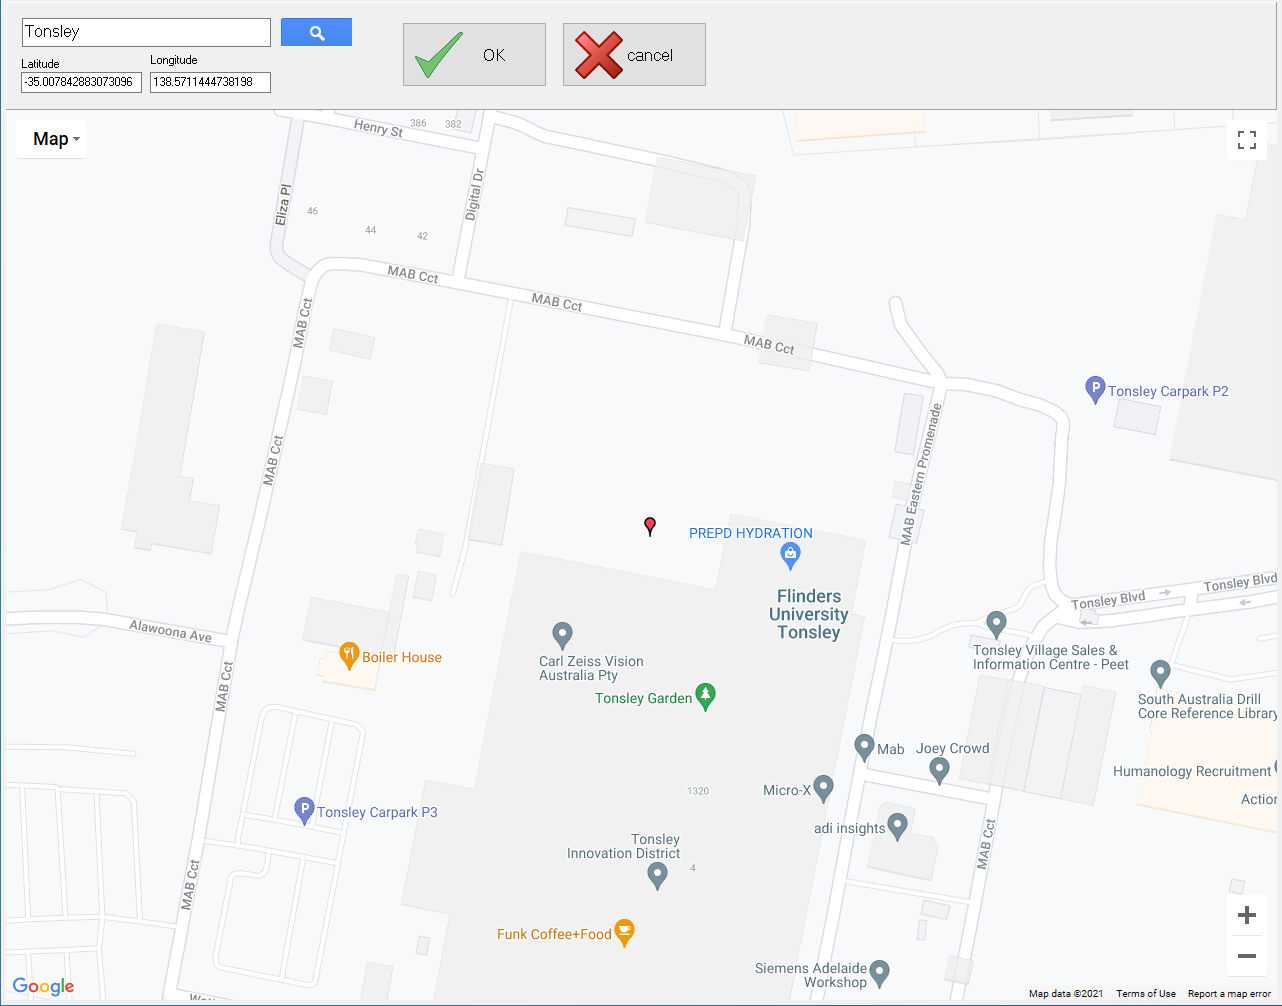
\includegraphics[width=12cm,keepaspectratio]{Figures/static coordinates setup.png}
        \caption{Using google maps within SatGen3 to choose a static coordinate to be used as desired spoof location}
    \label{fig:StaticCoordinate}
    \end{centering}
\end{figure}

\begin{figure}[ht]
    \begin{centering}
        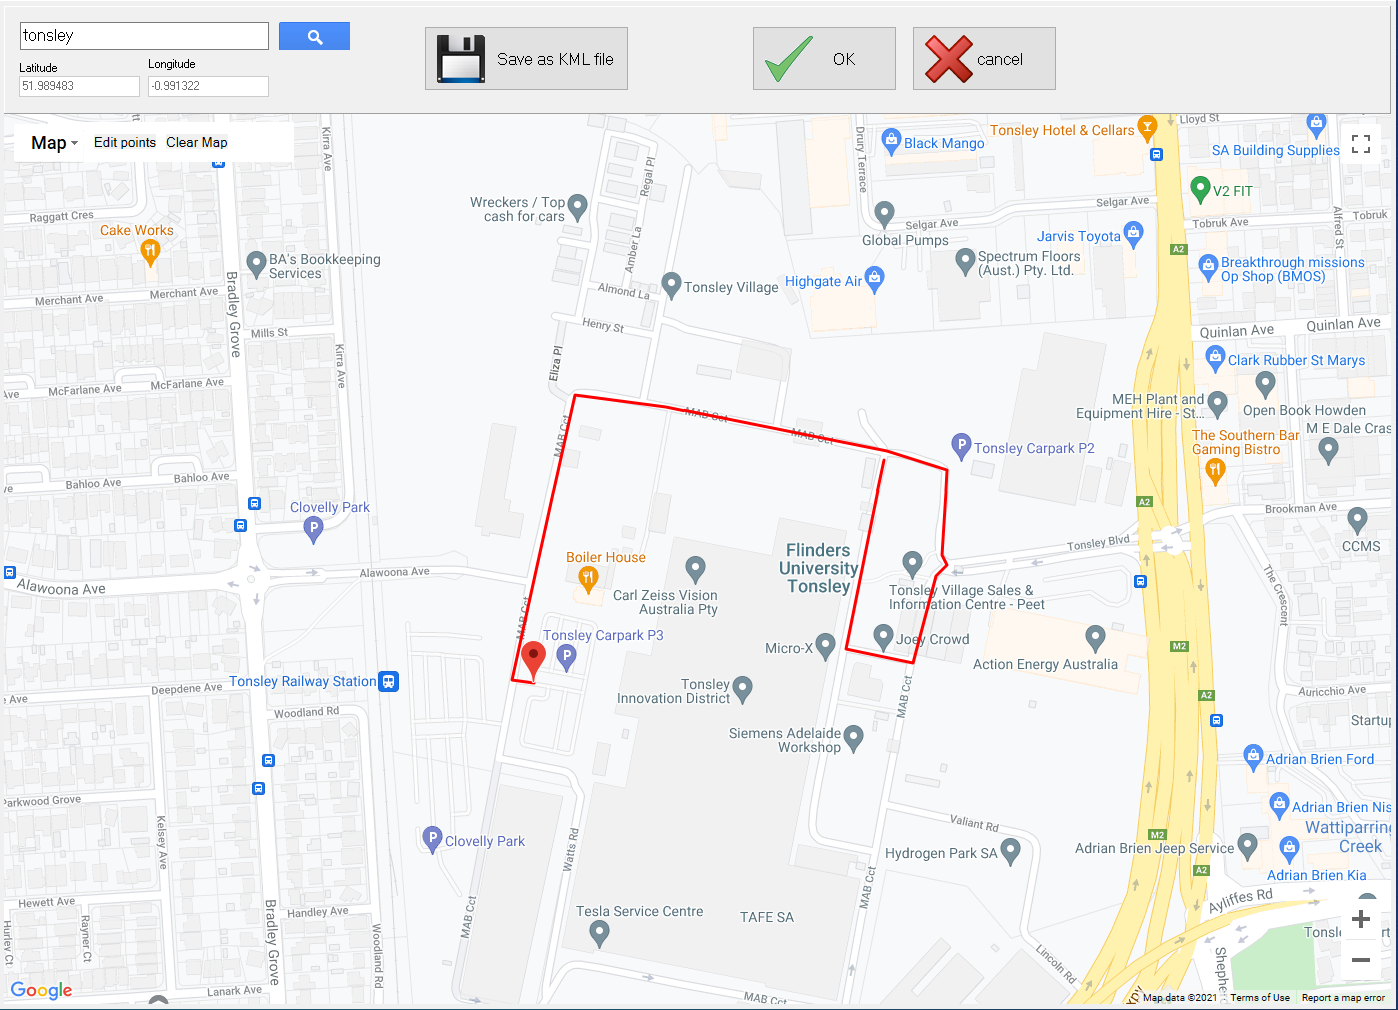
\includegraphics[width=12cm,keepaspectratio]{Figures/dynamic coordinates setup.png}
        \caption{Using google maps within SatGen3 to choose a set of coordiantes to be used as desired spoof path for a dynamic spoof attack}
    \label{fig:DynamicCoordinate}
    \end{centering}
\end{figure}

\subsection{Generate NMEA File} \label{subsec:NMEAFile}
The coordinate and NMEA file creation step is essentially the same step within the SatGen3 software package. Once the coordinate or path was chosen, it was a matter of
choosing to save the output as a txt file. An example of this is shown in Figure \ref{fig:StaticCoordinateNMEA}.

To generate the binary bitstream for use with an SDR RF front end a GGA NMEA data stream was created using the satgen3 software package. This NMEA stream was used to make
the binary file using the gps-sdr-sim command line interface program. SatGen3 replaces the need for capturing the raw GNSS signals or GGA sentence stream thus increasing
the flexilbilty of scenarios that can be tested. Although there is no guarentee that the simulated stream of information is going to be correct. Thus a capture replay
attack should still be considered as more reliable.

\begin{figure}[!ht]
    \begin{centering}
        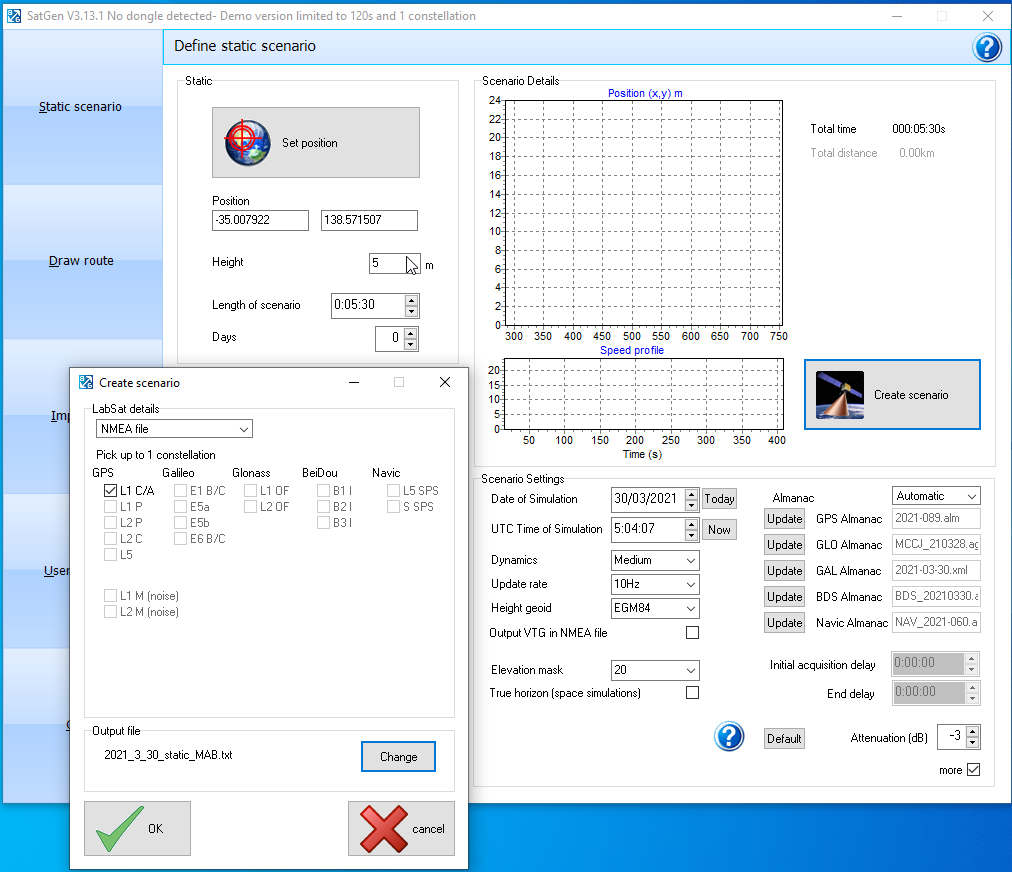
\includegraphics[width=12cm,keepaspectratio]{Figures/2021_03_30_static_MAB_setup.png}
        \caption{Using static coordinate to generate NMEA file}
    \label{fig:StaticCoordinateNMEA}
    \end{centering}
\end{figure}

\subsection{Download Ephemeris}
From the NASA website, hourly versions of the GPS constellation ephemeris, in the form of a RINEX file, are available. These are compiled into a daily file. These daily
files are available all the way from 1992. An account is required to access these files, but there are sample programs provided for retrieving
the files programically using different methods. A script was generated that was able to get the latest version from the website using Python. There were initially some
issues with getting the script to connect to the remote server to gain access to the files. It was found that there was a bug on linux with a certain version of openssl.
A newer version was manually installed and this solved the issue.

The downlaoded file was a compressed version of the text file, and thus it was required to be uncompressed using the tar program.

\subsection{Compile Signal Binary File}
The minimum requirements to compile a binary file using GPS-SDR-SIM was a source coordinate of some sort and the ephemeris for the desired date and time that the spoofer
will transmit. This did not need to match the date and time that the signal was being transmitted on.

Using this information, the place, time and ephemeris the program is able to calcaulate which of the satellites will be in view and what their expected psudo-ranges would
be. The signal modulation is applied wihtin the compilation of the file, simplifying the process of transmitting the file. 

\subsection{Transmit Signal}
Once the signal has been compiled into a binary file it is sent to the USRP SDR via GNURadio. GNURadio has an SDK that allows for text based programming. A script that was
capable of connecting to USRP devices automatically throught he UHD daemon was distributed with the gps-sdr-sim program. This was used to simplify the development
process. 

This was a simple program that connected the source file to the SDR via some simple blocks as shown in Figure \ref{fig:GNURadioSpoof}. The file is read 16bits at a time
into the "IShort to Complex" block. This converts the interleaved I/Q data into a complex file type which is then passed to the SDR via an amplifier block.

\begin{figure}[!ht]
    \begin{centering}
        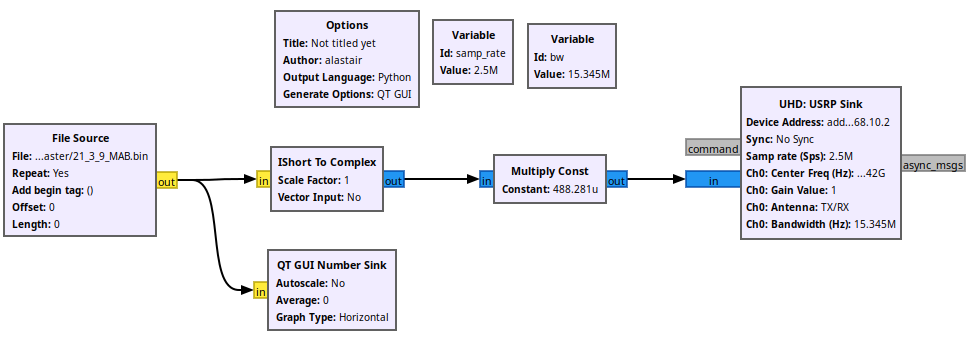
\includegraphics[width=14cm,keepaspectratio]{Figures/GNURadio_Spoofer.png}
        \caption{GNURadio flowchart for transmitting binary files with USRP}
    \label{fig:GNURadioSpoof}
    \end{centering}
\end{figure}

An important part of the transmission was that it needed to be performed within a faraday cage for legal purposes. This was discussed in section \ref{sec:FaraCage}.

\subsection{Log GPS Data}
To log the transmitted GPS signals from the SDR a COTS receiver and a smartphone were set up. The COTS receiver has a USB interface that outputs a stream of NMEA
senetences at a 1Hz frequency. This can be modified to 5Hz, but this was not required for these experiments. Using a script the USB port was opened and logged to a text
file. 

When using a smartphone Android was required for logging since the OS allows access to the raw properties of the recveived signal. There is also an intuituve applicaiton
"GNSS Logger" that allows for comprehensive visualistion of current GNSS tracking as well as the ability to log data. This data was logged to a text file using a non
standard layout, but there was an option to log the NMEA sentences as well.  

\subsection{Generate Graphs}
Once there was a log file, graphs were generated to visualise the various parameters of the location resolution as interpretated by the receiver. 
The generation of the graphs that make up the results section was done in python and was based upon the NMEA senetences logged from the receivers. GPS receivers have the
ability to check the validity of signals they recieve. When they are able to resolve a location the value of one of the fields within the RMC senntence is changed to
reflect this. The number of sentences before initial lock were counted. This was
used to determine the time to first fix of each test since it was known that the GPS receiver would output at 1Hz. Alterations would need to be made if the reciever was
outputting at a higher frequency. As such this should not be considered accurate and viewed as an estiamte only.

The carrier to noise ratio graphs were generated directly from the output of the GSV sentences. The SVID and associated $\frac{C}{N_0}$ ratios were stored as the value in
a key value pair. The key was a timestamp used to ensure each sentence was represented.

The latitude and longitude were retreiced from the GGA sentences.

Using the NMEA stream created in section \ref{subsec:NMEAFile} a desired plot was put on both the static and dynamic graphs. For the static graphs this reference was also
used as the origin when calculating the error of the calcualted location.

The error was calculated by finding the difference in latitude and longitude from the desired origin point and converting the $\Delta Lat$ and $\Delta Long$ into meters.
This assumes that the distances being dealt with are so small that they are essentially flat. Thus the equiations can be simplified to remove any angles.

The earth is not perfectly spherical therefore when converting latitude and longitude into x and y coordintes in meters the average of the polar plane and equitorial
planes were taken, as shown in equation \ref{eq:EarthCircumference}. The $\Delta x$ and $\Delta y$ values from Equation \ref{eq:deltaX} and \ref{eq:deltaY} represent
the error of the coordinate in the $x$ and $y$ direciton respectively.

When finding the total error value the law of Haversines was used. 

\begin{equation} 
    \begin{split} \label{eq:EarthCircumference}
        C_{Polar} = 40007.863 km \\ 
        C_{Equitorial} = 40075.017 km
    \end{split}
\end{equation}

\begin{equation} \label{eq:deltaX}
    \Delta x = \Delta Lat \times \frac{C_{Polar}}{\frac{2}{180}} \times 1000 m
\end{equation}

\begin{equation} \label{eq:deltaY}
    \Delta y = \Delta Long \times \frac{C_{Equitorial}}{\frac{4}{90}} \times 1000 m
\end{equation}

\begin{equation} \label{eq:Haversine}
    d = 2r \arcsin\left(\sqrt{\sin^2\left(\frac{\phi_2 - \phi_1}{2}\right) + \cos\left(\phi_1\right)\cos\left(\phi_2\right)\sin^2\left(\frac{\lambda_2 - \lambda_1}{2}\right)}\right)
\end{equation}
 
Below (Listing \ref{list:pythonHaversines}) is the implementation of the law of haversines in python used for the calcualtion of distance between two latitude and longitude points. The output of the function was stored
into an array and used to graph the total error over time.

% \begin{verbatim}
%     def latlon2m(lat1, long1, lat2, long2):
%         r = 6371000  
%         dLat = radians(lat2) - radians(lat1)
%         dLong = radians(long2) - radians(long1)
%         a = math.sin(dLat/2) * math.sin(dLat/2) + 
%             math.cos(radians(lat1)) * math.cos(radians(lat2)) *
%             math.sin(dLong/2) * math.sin(dLong/2)
%         d = 2*r*math.asin(math.sqrt(a))
%         return d
% \end{verbatim}

\begin{lstinputlisting}[language=Python, caption=Python implementation of the law of Haversines used to calculate the distance between two points on a sphere, firstline=23, lastline=29]{NMEAParse.py}
\label{list:pythonHaversines}
\end{lstinputlisting}


There is a PC companion application for the GNSS Logger app that allows for comprehensive
graphing and reports to be generated for a particular log file.

%----------------------------------------------------------------------------------------
%	SECTION 4
%----------------------------------------------------------------------------------------

%----------------------------------------------------------------------------------------
%	SECTION 5
%----------------------------------------------------------------------------------------



%----------------------------------------------------------------------------------------
%	SECTION 6
%----------------------------------------------------------------------------------------


%----------------------------------------------------------------------------------------
%	SECTION 7
%----------------------------------------------------------------------------------------

\section{Experiments}


\subsection{Static Spoofing}
Within this thesis static spoofing is defined as producing a signal that produces a calculated location that does not change over time. While in practise there was some
minor movement caused by the uncertainty in trilateration, this change in position is minor and within the range of error of GPS positioning.
Using the SatGen3 software a location was chosen as the spoof location. After setting the desired time and date of spoofing the scenario was created. THis 

\subsection{Dynamic Spoofing}
Dynamic spoofing refers to the production of a signal that when used to calcluate position, will be shown to change over time. The path traced by the receiver will be
set at the time of production of the binary file, see figure \ref{fig:21MarCBDDynamic}, but there will be perceived motion.

\subsection{Real-Time Spoofing}
Due to time constraints a real-time algorithm was not produced as part of this project. However, utelising the open source projects that have been used to complete this
thesis it would be probable to be able to create a real time spoofing device that would be able to react to the positional changes of the receiver instead of following a
pre-determined path when generating the binary file. The signals generation algorithm could be ported to a GNURadio block in C++ to allow for easy access to real-time GPS
signal spoofing. If an SDR is a full duplex radio, such is the case for the USRP N210, then one port can be receiveing the real GNSS signal and the other can be
transmitting the spoofed signal. Care would need to be taken in the set up of this arrangement since any transmitted signal would also be picked up by the reciving
antenna. Therefore a directional transmitting antenna and physical disctance should be employed to allow for legitimate GNSS signals to reach the reciever port. 

%----------------------------------------------------------------------------------------
%	SECTION 8
%----------------------------------------------------------------------------------------

\section{Parameters required for successful spoofing}
\todo{add screen shots of steps required to generate binary file}
Due to the internal workings of the USRP, there needs to be an integer ratio between the clock rate and sample rate. Therefore is was required that the sample frequency
was set to 2.5Msps instead of the default 2.6Msps that the software would normally use.

\begin{figure}[h]
    \begin{centering}
        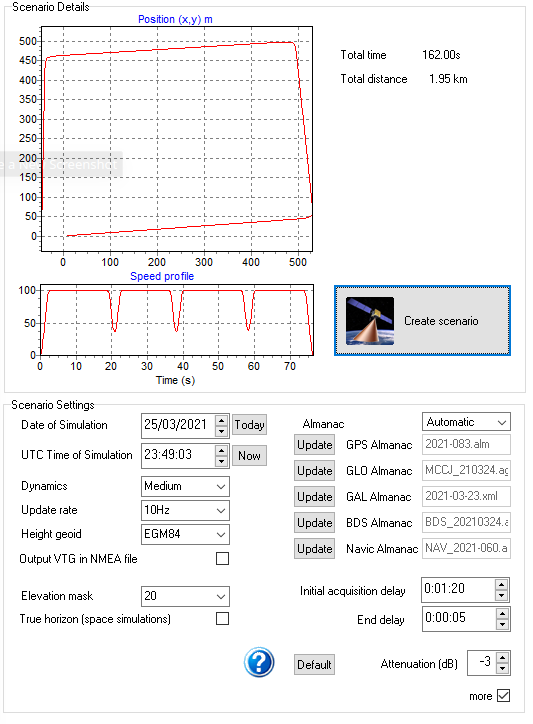
\includegraphics[width=14cm, keepaspectratio]{Figures/21-3-25_cbd_dynamic_setup.png}
        \caption{Settings of SatGen3 used to generate the dynamic path loop around Adelaide CBD. There is a graph that shows the offset from the origin and speed over the journey}
    \label{fig:21MarCBDDynamic}
    \end{centering}
\end{figure}

%----------------------------------------------------------------------------------------
%	SECTION 9
%----------------------------------------------------------------------------------------

\section{SDR Setup for GNSS Reception}
Reception of GNSS signals is a compliated process which involves sychronising time values and solving simultaneous equtations for position, therefore it was decided that
the opensource program GNSS-SDR would be used to perform all of these functions. This sofware has been built over a number of years and is able to receive different GNSS
signals and translate them into position.

The hardware setup for this was different. Since the signal strength of a GNSS transmission is so low when it reaches the earths surface ($\approx -160dBm$) an active
antenna is typically requied for best performance, especially if there is no clear view of the sky or if there are many buildings that add multipath signals into
consideration.
 
% % Chapter Template

\chapter{Chapter Title Here} % Main chapter title

\label{Chapter5} % Change X to a consecutive number; for referencing this chapter elsewhere, use \ref{ChapterX}

%----------------------------------------------------------------------------------------
%	SECTION 1
%----------------------------------------------------------------------------------------
 
% % Chapter Template

\chapter{Discussion} % Main chapter title

\label{Chapter6} % Change X to a consecutive number; for referencing this chapter elsewhere, use \ref{ChapterX}
This section will discuss the results gathered from the previous section \ref{Chapter5}. Any broad findings or trends will be noted and explanations of why results are
the way they are.

%----------------------------------------------------------------------------------------
%	SECTION 1
%----------------------------------------------------------------------------------------

\section{Results}
Initially it was decided that the locations that would be spoofed would be locations that are not easily accessible as a means of proving the validity of the results.
This was made easier due to the ongoing pandemic. Although this idea was later changed to make it easier to compare with real signals if needed.

Using the developed workflow, it was simple to create and deploy spoofing attacks for any location and at any elapsed time within minutes. This includes static or dynamic
spoofing attacks. Not enough time was invested into the reception of GNSS signals and thus meaconing attacks were not performed. The GPS-SDR-sim program was able to
estimate and simulate the ionic effects. While it is clear that this method resulted in successful spoofing attacks, the hypothesis is that having a received signal that includes ionic delays
and other interference would make it easier to fool more complicated receivers. Further testing and investigations should be carried out to find the answer to this. 

The results from the static Antarctica spoof attack, specifically the carrier to noise graphs show a high number of unique SVIDs. Based on the number of satellites in the
GPS constellation this must be an error. Although there was no explanation for the error since the resultant location was correct. One hypothesis was that the compilation
software added some incorrect data. Another is the prevalence of SBAS satellites. There was a known issue for some time with the Faraday cage where stray EM waves were
getting in. This would explain the consistency in which SVID 193 appears. From \cite{RN67} it can be seen that SVID 193 is a QZSS satellite. These satellites orbit over
Australia and part of Asia.

Consistently for both static and dynamic spoofing the $\frac{C}{N_0}$ ratio was a high value (between 40 and 50 dBHz). During experimentation it was found that authentic
GPS signals would be received with more variable $\frac{C}{N_0}$ ratio but with an average of arround 30dBHz. This discrepency can be attributed to a combination of the
controlled environment of the Faraday cage as well as the reletive distance between the spoofer and victim. In theory the spoofed $\frac{C}{N_0}$ ratio could be higher,
but during compilation estimated Ionospheric effects are included. This shows that there is still room for improvement for the GPS-SDR-sim software, especially if it is
to be used in controlled environments for testing purposes. Just from the $\frac{C}{N_0}$ ratio graphs the spoofed signals are easy to identify.

On the $\frac{C}{N_0}$ ratio graphs there were consistently more SVIDs than expected. The trend was that static spoof attacks had more SVIDs than the dynamic spoofs, with
the most coming from the Antarctic spoof attack. It can also be seen that the length of attack was longest for the Antarctic spoof, which may account for this
discrepency. Even still, the MAB static spoof included more than expected SVIDs.

SDRs are very sensitive to the processing pipeline of the computer that they are connected to. It is not uncommon to receive an under run error (where 'U' is printed to the
output) when transmitting a signal with high SPS (samples per second). This error is caused by the host computer not being able to feed the data to the radio quickly
enough.

This was solved by increasing the UDP buffer size manually to at least the sample rate, and over for better results. From limited experimentation this completely resolved the issue, and opened up
opportunities to perform spoofing with low powered embedded devices like the Raspberry Pi single board computer.

\section{Future Work}
All of the tests that have been conducted for use in this thesis have either been generating a signal based off a predetermined location (coordinate) or a predetermined
path (group of connected coordinates). None of these options have a mechanism for position feedback. For example you cannot create a signal that has a linear offset from
the actual position using these methods. This is something that could be achieved through combination and modification of the existing open source projects used in this
thesis. This would allow for properly real-time GPS spoofing, and could be extended further to have intelligent algorithms.

Current methods, as detailed in Chapter \ref{Chapter4}, requires downloading the Ephemeris for the date and time of the proposed spoofing attack. This makes real-time spoofing
attacks not possible since there is a delay between the current time and the associated ephemeris. A potential fix for this could be to perform some analysis on the
orbits of each satellite within the constellation over an arbitrary period of time to create a machine learning algorithm. This algorithm would be able to predict the
location of the satellites ahead of time, thus binaries could be compiled for future attacks, or could be used for real-time attacks without the need for downloading/
retrieving the ephemeris from legitimate sources.

The logging program could be extended to provide real time feedback on position and signal quality. This would be achieved by implementing the serial connection within
the Python code itself rather than relying on the logging function of screen.
Extended to work on anti-spoofing for PhD. If there was more time for this project, a software based anti spoofing program would have been easy to implement based
on the $\frac{C}{N_0}$ ratio alone. This could be implemtnted in conjucntion with real time graphing as mentioned above.

The hardware used for this project was successfully used for spoofing attacks, however, the software must be altered in order to achieve the accurate results that were
expected of the project. However ensuring software capabilities was out of the scope of this thesis.
% % Chapter Template

\chapter{Conclusion} % Main chapter title

\label{Chapter7} % Change X to a consecutive number; for referencing this chapter elsewhere, use \ref{ChapterX}

%----------------------------------------------------------------------------------------
%	SECTION 1
%----------------------------------------------------------------------------------------
One of the aims of this project was to create hardware that is capable of successfully spoofing a GPS receiver. From the results it can be seen that the method of
spoofing using signals generated from coordinates was successful. There were issues that impacted the results at times, however, these were overcome to produce good
results in both static and dynamic spoofing. The hardware that was used for this is capable of performing any spoofing attack, however the
software was not cable to produce the results at times, where anti-spoofing was at play.
Overall the accuracy of the position gathered from the GPS receivers was poorer than expected, although
to be able to spoof anything at all was considered a success. Given these results were gathered in a controlled environment more care will need to be taken if
performing these experiments in the field. The project was able to provide a foundation for which further research into GNSS attack and defence strategies can be
performed. SDR devices are prevalent in EW research due to their combination of hardware level performance and software level flexibility. This will allow for further
research into other areas of EW.
There were no results gathered from performing Meaconing attacks since the GPS signal reception was unsuccessful and therefore signal capture was unavailable.

Through this thesis it has been shown that with relatively low amounts of technical knowledge successful spoofing attacks can be performed. Some basic computer literacy
was required in order to install and configure the software needed to perform the attacks. The simplest way of using the software is with Linux which does add a level of
difficulty.
Moving forward into the future the software could be given a graphical interface and integrated into one software package, or simplify the transmission interface and use
pre compiled binaries.
% % Chapter Template

\chapter{Chapter Title Here} % Main chapter title

\label{Chapter8} % Change X to a consecutive number; for referencing this chapter elsewhere, use \ref{ChapterX}

%----------------------------------------------------------------------------------------
%	SECTION 1
%----------------------------------------------------------------------------------------

%----------------------------------------------------------------------------------------
%	THESIS CONTENT - APPENDICES
%----------------------------------------------------------------------------------------

\appendix % Cue to tell LaTeX that the following "chapters" are Appendices

% Include the appendices of the thesis as separate files from the Appendices folder
% Uncomment the lines as you write the Appendices

% Appendix Template

\chapter{Project Code} % Main appendix title

\label{AppendixA} % Change X to a consecutive letter; for referencing this appendix elsewhere, use \ref{AppendixX}

\textbf{\emph{This section will include all of the code that has been written for this project, including the code to fetch the ephemeris and the code to plot the
position and signal quality}}

\section{GPS Position and Signal Quality}
\textbf{Filename:} NMEA.py\\
\textbf{Description:} This code will take a NMEA file as input and calculate the time to first fix, then plot the carrier to noise ratio of every satellite that was
within view of the receiver, then plot the position given the output of the GPS receiver.

\begin{verbatim}
    insert code here
\end{verbatim}

%% Appendix Template

\chapter{GPS Receiver NMEA Sentence ouput} % Main appendix title

\label{AppendixB} % Change X to a consecutive letter; for referencing this appendix elsewhere, use \ref{AppendixX}

\section{Receiver Output}
Below is a snippet of the output from the GPS recevier unit used for testing.

\section{File used for generating binary}
Below is a snippet of the NMEA file that was used to generate the binary file.
%\include{Appendices/AppendixC}

%----------------------------------------------------------------------------------------
%	BIBLIOGRAPHY
%----------------------------------------------------------------------------------------

\printbibliography
\end{document}  
